\documentclass{article}
\usepackage[english]{babel}
\usepackage[margin=1in, landscape]{geometry}
\usepackage{amssymb}
\usepackage{amsfonts}
\usepackage{amsmath}
\usepackage{multicol}
\usepackage{multirow}
\usepackage{calc}
\usepackage{ifthen}
\usepackage{hyperref}
\usepackage{lastpage}
\usepackage{fancyhdr}
\usepackage{accents}
\usepackage{changepage}
\usepackage{graphicx}
\usepackage{tikz}
\usepackage{tcolorbox}
\usepackage{xcolor}
\usepackage{circuitikz}
\usepackage[parfill]{parskip}
\usepackage[toc]{appendix}
\usepackage[acronym, toc]{glossaries}
\usepackage{steinmetz}
\usepackage[style=ieee]{biblatex}
\usepackage[document]{ragged2e}
\usepackage{babel}
\usepackage{tabularx}

\title{\textbf{Getting Started with Git \& GitHub on Windows}}
\author{\href{https://github.com/th1622EE?tab=repositories}{Tim Holden}}
\date{\today}

\hypersetup
{
    colorlinks=true,
    linkcolor=black,
    filecolor=magenta,      
    urlcolor=blue,
    pdfpagemode=FullScreen,
    citecolor=black,
}

\addbibresource{bibliography}

\makeglossaries
%%%%%%%%%%%%%%%%%%%%%%%%%%%%%%%%%%%%%%%%%%%%%%%%%%%%%%%%%%%%%%%%%%%%%%%%%%%%%%%%%%%%%%%%%%%%%%%%%
% Glossary Entries
%%%%%%%%%%%%%%%%%%%%%%%%%%%%%%%%%%%%%%%%%%%%%%%%%%%%%%%%%%%%%%%%%%%%%%%%%%%%%%%%%%%%%%%%%%%%%%%%%
\newglossaryentry{efficiency}
{
    name = efficiency,
    description = {a measure of how well an antenna converts electric power (i.e., voltage, current, power) into radiated electromagnetic power (i.e, electromagnetic waves).}
}

\newglossaryentry{bandwidth}
{
    name = bandwidth,
    description = {the span of frequencies over which certain characteristics of its performance fall within an acceptable range.}
}

%%%%%%%%%%%%%%%%%%%%%%%%%%%%%%%%%%%%%%%%%%%%%%%%%%%%%%%%%%%%%%%%%%%%%%%%%%%%%%%%%%%%%%%%%%%%%%%%%
% Acronym Entries
%%%%%%%%%%%%%%%%%%%%%%%%%%%%%%%%%%%%%%%%%%%%%%%%%%%%%%%%%%%%%%%%%%%%%%%%%%%%%%%%%%%%%%%%%%%%%%%%%
\newacronym{plf}{PLF}{Polarization Loss Factor}


\begin{document}

\begin{titlepage}
    \maketitle
    \thispagestyle{empty}
    \newpage
\end{titlepage}

\tableofcontents
%\listoftables
\listoffigures
\newpage

\section{Introduction}
Antenna \textit{Figures of Merit} are the measurable characteristics of an antenna by which an antenna would be designed for a specific application. These characteristics include physical data, but more specifically relate to the performance of the antenna to include but not limited to radiation pattern, gain, efficiency, frequency of operation, bandwidth, input impedance, et al. Almost all of the performance characteristics of a given antenna will vary with frequency to include the radiation pattern, the strength of that radiation, the polarization of the radiated wave, the input impedance of the antenna, efficiency of the antenna, bandwidth, et al. This document was created as a reference to \textit{figures of merit} specific to antenna theory and design.

\section{Antenna Efficiency}
The \gls{efficiency} of an antenna is a measure of how well an antenna converts electric power (i.e., voltage, current, power) into radiated electromagnetic power (i.e., electromagnetic waves). For the purpose of simplifying this explanation refer to the simplified circuit representing a network that feeds power to the antenna:

\begin{figure}[h!]
    \centering
    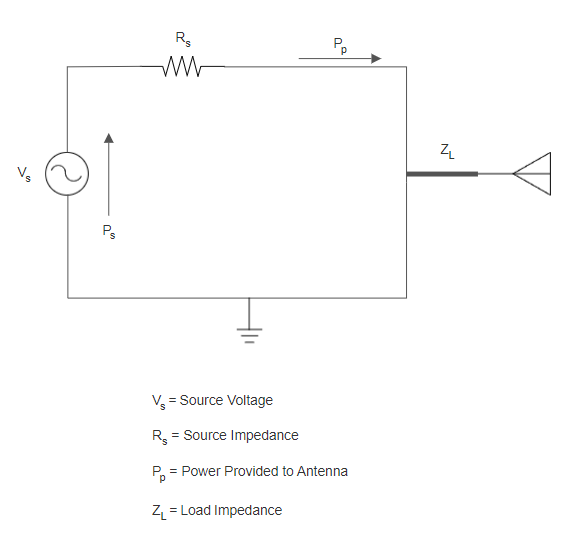
\includegraphics[scale=0.75]{images/simpleAntennaCircuit.png}
    \caption{Simplified Antenna Feed Network Circuit Diagram}
    \label{fig:1}
\end{figure}
\newpage

The above network model (\ref{fig:1}) is representative of a source network (commonly referred to as a generator network) lumped together into a singular source voltage $V_s$ and source impedance $R_s$ on the left, which provides power to the load $Z_L$ (i.e., the antenna) over a feed line with a defined characteristic impedance $Z_0$, and ultimately converts the electrical power into radiated electromagnetic power transmit as electromagnetic waves. Given a defined \textit{source voltage}, we can calculate \textit{source power} with respect to \textit{source voltage} as follows:

\begin{equation}\label{sourcePower}
    P_s = \dfrac{V_s^2}{R_s}
\end{equation}

\subsection{The Theoretical Best Case Efficiency}
The efficiency of an antenna performs optimally when the source impedance $R_s$ is perfectly matched to the load impedance $Z_L$ (i.e., antenna input impedance $Z_{in}$), and the characteristic impedance $Z_0$ of the feed line. This is mathematically defined as follows:

\begin{equation}\label{matchedCondition}
    R_s = Z_{in} = Z_0
\end{equation}

Assuming the source voltage $V_s$ is 10 \textbf{V}, and the conditions defined in ($\ref{matchedCondition}$) are met, using equation ($\ref{sourcePower}$) above, the source power $P_s$ would be as follows:

\begin{equation*}
    P_s = \dfrac{10^2}{50} = 2 \textbf{W}
\end{equation*}

Similarly, the \textit{power provided} to the antenna can be calculated as a function of the \textit{source voltage} $V_s$ and the sum of the \textit{source impedance} $R_s$ and the \textit{load impedance} as follows:

\begin{equation}\label{powerProvided}
    P_p = \dfrac{V_s^2}{R_s + Z_L} = \dfrac{10^2}{50 + 50} = 1 \textbf{W}
\end{equation}

It is important to note the \textit{power provided} $P_p$ to the antenna is the \textit{source power} minus the \textit{power} lost due to the voltage drops across the \textit{source impedance} \textbf{and} \textit{load impedance} of the network. Furthermore, \textbf{IFF} the load, line, and source impedances are perfectly matched as defined in equation ($\ref{matchedCondition}$) above will the antenna efficiency perform at its theoretically optimal limit. This implies that \textbf{half} of the \textit{source power} will be absorbed by the network, and \textbf{half} the \textit{source power} will be provided to the antenna. This is defined mathematically as follows:

\begin{equation*}
    P_p = 0.5P_s
\end{equation*}

\subsection{Considerations for Efficiency in Design}
Given the optimal efficiency of an antenna at $0.5P_s$, it is extremely important when designing an antenna to consider factors which could further diminish the efficiency of the antenna. There are several reasons antenna efficiency could be further decreased as inefficiencies in design are introduced. The following subsections describe the most significant factors impacting antenna efficiency which should be considered in the design phase of a system.

\subsubsection{Impedance Mismatch Efficiency}
The most common and likely most significant reason for reduced efficiency is when the impedance of the feed network is not matched to the impedance of the antenna resulting in the reflection of power back toward the generator due to the impedance discontinuities (i.e., mismatched networks). In this specific case, the power absorbed by/input to the antenna would be less than the power provided to the antenna:

\begin{equation*}
    P_{in} < P_p
\end{equation*}

This is known as \textit{Impedance Mismatch Efficiency} and defines a quantitative error as the ratio of the input power to the power provided to the antenna. This is mathematically defined as follows:

\begin{equation}\label{mismatchEfficiency}
    e_r = \dfrac{P_{in}}{P_p}
\end{equation}

Therefore, the actual \textit{input power} to the antenna in this specific case is defined mathematically as follows:

\begin{equation*}
    P_{in} = P_p e_r
\end{equation*}

\subsubsection{Radiation Efficiency}
Another common reason inefficiencies are introduced results from the use of low-quality (i.e., lossy) materials and/or components. For example, if the antenna conductors are slightly resistive, or the dielectrics are slightly conductive, the \textit{input power} $P_{in}$ to the antenna will be partially dissipated in the body of the antenna as \textit{ohmic losses} which ultimately reduces the amount of power which can and/or will be radiated by the antenna. This is referred to as the \textit{radiation efficiency} of the antenna and mathematically defined as follows:

\begin{equation}\label{radiationEfficiency}
    e_{cd} = \dfrac{P_{rad}}{P_{in}}
\end{equation}

The \textit{radiation efficiency} is equal to the ratio of power radiated $P_{rad}$ by the antenna to the power input $P_{in}$ at its port. Therefore, the power radiated from the antenna is defined mathematically as follows:

\begin{equation*}
    P_{rad} = P_{in} e_{cd}
\end{equation*}

\subsubsection{Total Antenna Efficiency}
The \textit{total antenna efficiency} is the error in efficiency when \textit{antenna mismatch efficiency} and \textit{radiation efficiency} are combined. This is the ratio of the power radiated $P_{rad}$ to the power provided $P_p$ to the antenna by the source and defined mathematically as follows:

\begin{equation}\label{totalEfficiency}
    e_0 = e_{cd} e_r = \dfrac{P_{rad}}{P_p} = \left[ \left( \dfrac{P_{rad}}{P_{in}} \right) \left( \dfrac{P_{in}}{P_p} \right) \right]
\end{equation}

Therefore, the power radiated $P_{rad}$ by the antenna relative to the \textit{total antenna efficiency} is defined mathematically as follows:

\begin{equation*}
    P_{rad} = e_0 P_p
\end{equation*}

\subsubsection{Polarization Loss Factor}
It is also worth nothing that only the portion of the radiated power that conforms to the desired polarization is usable. Therefore, any power radiated in a different polarization (cross-polarization power) could be considered as a loss. To include this type of loss in the design we can add what is known as the \acrlong{plf} (\acrshort{plf}). The \acrshort{plf} is the ratio of power in the desired polarization $P'_{rad}$ to the total radiated power $P_{rad}$. For a linear radiator the \acrshort{plf} is defined mathematically as follows:

\begin{equation}\label{plf}
    PLF = \cos^2{\phi}
\end{equation}

Where $\phi$ is the difference in the angle between the desired polarization and the actual polarization. For example, if vertical polarization is desired, but the antenna is radiating at a $45\circ$ angle, the total usable power is defined mathematically as follows:

\begin{equation*}
    P'_{rad} = \cos^2{45\circ} P_{rad}
\end{equation*}

When considering this type of loss in the design of the antenna, the total usable (desired polarization == actual polarization) radiated power is defined mathematically as follows:

\begin{equation*}
    P'_{rad} = e_0 P_p PLF
\end{equation*}

\subsection{Summary of Antenna Efficiency Considerations}
In the design of an antenna, the following considerations are imperative in maximizing antenna efficiency:
    \begin{enumerate}
        \item The antenna input impedance matches the impedance of the feed network.
        \item The materials used in building the antenna are low loss at the desired operating frequencies.
        \item The polarization of the antenna is appropriate to the application.
    \end{enumerate}

\section{Antenna Bandwidth}
Antenna \gls{bandwidth} is the span of frequencies over which certain characteristics of its performance fall within an acceptable range.

\newpage
\clearpage
\printglossary
\printglossary[type=\acronymtype]

\end{document}